\documentclass[sigplan,anonymous,review]{acmart}

\usepackage{authorcomments}
\usepackage{listings}
\usepackage{algorithm}
\usepackage{algpseudocode}
\usepackage{xspace}
\usepackage{paralist}


\lstset{language=R}
\definecolor{LightGray}{rgb}{.92,.92,.92}
\definecolor{Gray}{rgb}{.3,.3,.3}
\definecolor{DarkGray}{rgb}{.5,.5,.5}
\lstset{ %
  columns=flexible,
  captionpos=b,
  frame=single,
  framerule=0pt,
  tabsize=2,
  belowskip=0.5em,
  backgroundcolor=\color{LightGray},
  basicstyle=\small\ttfamily,
  emphstyle=,
  keywordstyle=,
  commentstyle=\color{Gray}\em,
  stringstyle=\color{Gray},
  numbers=left,
  showstringspaces=false
}
\lstdefinestyle{R}{ %
  language=R,
  morekeywords={assign, delayedAssign},
  deletekeywords={env, equal, c, runif, trace, args, exp, t, all},
  breaklines=true
}
\lstdefinestyle{Rin}{ %
  style=R,
  breaklines=false
}


\newcommand{\tool}{\texttt{signatr}\xspace}
\newcommand{\numFnsCaseStudy}{20\xspace}
\newcommand{\numPkgsScaleStudy}{20\xspace}
\newcommand{\code}[1]{{\lstinline[style=Rin]!#1!}\xspace}

% For algorithmcx
\algnewcommand{\LineComment}[1]{\State \(\triangleright\) #1}
\newcommand{\DBFileSize}{287.17 GB\xspace}
\newcommand{\DBValuesRnd}{39.4M\xspace}
\newcommand{\DBValues}{39,425,582\xspace}
\newcommand{\DBNumPackagesRnd}{652\xspace}
\newcommand{\DBNumPackages}{652\xspace}
\newcommand{\DBNumFunctionsRnd}{38.1K\xspace}
\newcommand{\DBNumFunctions}{38,109\xspace}
\newcommand{\DBNumSourceFilesRnd}{17.5K\xspace}
\newcommand{\DBNumSourceFiles}{17,463\xspace}
\newcommand{\DBSourceLinesOfCodeRnd}{389.7K\xspace}
\newcommand{\DBSourceLinesOfCode}{389,740\xspace}

\newcommand{\UFTracingBudgetRnd}{5K\xspace}
\newcommand{\UFTracingBudget}{5,000\xspace}
\newcommand{\UFNumTracesRnd}{12.1M\xspace}
\newcommand{\UFNumTraces}{12,115,000\xspace}
\newcommand{\UFNumSuccessTracesRnd}{2.1M\xspace}
\newcommand{\UFNumSuccessTraces}{2,062,046\xspace}
\newcommand{\UFRatioSuccessTraces}{17\%\xspace}
\newcommand{\UFNumPackagesRnd}{78\xspace}
\newcommand{\UFNumPackages}{78\xspace}
\newcommand{\UFNumFunctionsRnd}{2.4K\xspace}
\newcommand{\UFNumFunctions}{2,423\xspace}
\newcommand{\UFNumOfCrashedRSessionsRnd}{201\xspace}
\newcommand{\UFNumOfCrashedRSessions}{201\xspace}
\newcommand{\UFNumSuccessPackagesRnd}{69\xspace}
\newcommand{\UFNumSuccessPackages}{69\xspace}
\newcommand{\UFNumSuccessFunctionsRnd}{1.2K\xspace}
\newcommand{\UFNumSuccessFunctions}{1,228\xspace}
\newcommand{\UFNumFunctionSignatrSignatureRnd}{1.1K\xspace}
\newcommand{\UFNumFunctionSignatrSignature}{1,113\xspace}
\newcommand{\UFAvgNewSignatrSignatureRnd}{707.7\xspace}
\newcommand{\UFAvgNewSignatrSignature}{707.7\xspace}
\newcommand{\UFAvgNewSignatrSignatureRatioRnd}{213\xspace}
\newcommand{\UFAvgNewSignatrSignatureRatio}{213\xspace}
\newcommand{\UFBaselineSignaturesRnd}{8.3K\xspace}
\newcommand{\UFBaselineSignatures}{8,272\xspace}
\newcommand{\UFSignatrSignaturesRnd}{787.7K\xspace}
\newcommand{\UFSignatrSignatures}{787,696\xspace}
\newcommand{\UFSharedSignatureRnd}{834\xspace}
\newcommand{\UFSharedSignature}{834\xspace}
\newcommand{\UFSharedSignatureFunctionRnd}{432\xspace}
\newcommand{\UFSharedSignatureFunction}{432\xspace}
\newcommand{\UFSignatrBaselineSignaturesRatioRnd}{95.2\xspace}
\newcommand{\UFSignatrBaselineSignaturesRatio}{95.2\xspace}
\newcommand{\UFNumMissingFunctionSignatrRnd}{1.3K\xspace}
\newcommand{\UFNumMissingFunctionSignatr}{1,310\xspace}
\newcommand{\UFNumMissingFunctionSignatrRatio}{54.1\%\xspace}
\newcommand{\UFNumFunctionSignatrSignatureRatio}{45.9\%\xspace}
\newcommand{\UFNumFunctionBaselineSignatureRnd}{2K\xspace}
\newcommand{\UFNumFunctionBaselineSignature}{2,038\xspace}
\newcommand{\UFNumFunctionBaselineSignatureRatio}{84.1\%\xspace}
\newcommand{\UFNumErrorMessagesRnd}{789.9K\xspace}
\newcommand{\UFNumErrorMessages}{789,896\xspace}


\begin{document}

\title{\tool: A Data-Driven Fuzzing Tool for R}

\begin{abstract}

Fuzzers are automated tools that test functions by generating novel inputs, calling the function with the inputs, and observing their behavior.
There exist myriad fuzzing tools for many programming languages, and they have been used to uncover novel bugs in various application domains.
That said, fuzzing in the context of \textit{dynamic} languages is tricky, as the shape of user-defined data is difficult to automatically determine ahead-of-time.
In this work, we propose a novel feedback-driven blackbox fuzzing approach which draws function inputs from a database populated with values observed by running a large corpus of existing code; we implement this approach in a tool called \tool for the R programming language.
% The database backing \tool is comprised of \DBValuesRnd unique values obtained from \DBSourceLinesOfCodeRnd lines of R code. % <-- Not sure that we need this.

As an application of this technique in the context of language design, we stress-test one of the proposed type system designs for R, which was inspired by a corpus analysis of R code.
As an argument in favor of their design, authors present function types inferred from running R code, and this paper reports on an experiment where \tool was run on \UFNumFunctions of those functions R functions, generating \UFSignatrAdditionalSignatures (\UFSignatrAdditionalSignaturesRatio times) more unique call signatures than were obtained from running existing code alone.

\end{abstract}

\maketitle

\section{Introduction}
\label{sec:introduction}

% Fuzzing is a thing, and it is useful.
Fuzzing has established itself as useful technique for test generation and security.
At a high level, fuzzers are automated testing tools that call programs with randomly generated inputs in an effort to uncover bugs, locate security vulnerabilities, generate new software tests, etc.
\AT{Say a bit more.}

% Dynamic language semantics make it difficult to fuzz in them.
While fuzzing has seen widespread adoption across many different programming languages, \textit{dynamically typed} programming languages such as Python, JavaScript, and R pose unique challenges which revolve around the idea that dynamically typed code tends not to result in runtime errors.
Essentially, the semantics of these languages is very permissive: for instance, accessing a non-existent field of an object in JavaScript yields the value {\tt undefined}, and basic functions in R will readily coerce values whose types do not match (and the coercion rules depend on the function in question).
More broadly, the lack of static types at function boundaries that are checked ahead-of-time can cause \AT{\ldots}

% Value types are hard to come by.
Another important challenge facing general-purpose fuzzing in the context of dynamic languages is the difficulty in obtaining complex values automatically.
In a statically typed language like Java, the shapes of user-defined objects can be inferred from a static class definition, and this not always possible in, e.g., dynamic prototype-based inheritance in JavaScript, or dynamic object definition in R.
Thus, an effective fuzzer would need to be manually equipped with the ability to create values of these complex types, which places an undue burden on developers.

% In this paper, ...
To get around this, we propose a general-purpose approach for fuzzing that relies on a database of values observed during the execution of real code.
We develop a tracer that collects information about function calls and values observed during code execution, and this information is stored in a database with an expressive query API.
We propose a fuzzing approach that relies on this database to generate new function inputs based on massive amounts of existing observed values.
This approach is implemented in a tool called \tool for the R programming language.

% Retrofitted.
\AT{Sort of comes out of nowhere.}
As a use case for our tool, we argue that a general-purpose fuzzer can aid data-driven retrofitted type system designers by providing them with unexpected but valid inputs for existing functions.
We develop an approach for synthesizing the results of fuzzing into a type signature for a function, entirely parameterized over a type system expressed as (1) a function to infer the type of a value, and (2) a function to determine if one type is a subtype of another.


In summary, the contributions of this paper are:
%
\begin{inparaenum}[(1)]
    \item a novel fuzzing technique relying on a database of observed values;
    \item an implementation of this approach in a tool called \tool for the R programming language; and
    \item a use case for \tool where it is used to generate many yet unseen, successful inputs for thousands of R functions.
\end{inparaenum} 

% Using the tool, we generate a value database \TODO{DB stats} and use it to fuzz trace types for \TODO{experiment stats}.
% We find \TODO{result stats}.
% %
The tool is open source and is available online alongside the data set used for this paper.


\FK{Typer paper gave us a foundation for an eventual type system for R.
It was trying to answer the quetions about:
(1) What expressive power is needed to accurately type R code? 
(2) Which type system is the R community willing to adopt?
In this paper we want to move one step closer to the actual type system.
Some questions:
(1) Are the traces we used before enough? The reason for this question is that one of the key point of dynamic languages is that they try to "fail" as little as possible - they keep going even if the shape of the data is not exactly what it should be. So the question is what all a function can take and ideally what still makes sense (though this is much harder to get without oracles),
(2) How polymorphic are the polymorphic functions that we see?
(3) What should be the type base functions?
(4) How about S3 dispatch and coertion?
}


\FK{Few things to mention (random notes): (1) we are looking at type systems for users (not machines), e.g. a user would likely prefer an arrow of union while a compiler would do better with a union of arrows.
(2) R is somewhat different from Python and JS in the way that it lacks any sort of modules (modulo S4,...). In JS/Python we have classes and objects in the OOP style - that is not what we have in R - or at least not in the same sense. The S3 generics are tricky because they encapsulate too many different objects - it is really an adhoc polymorphims, much like operation overloading. (4) This is second paper in the series of papers whose goal is to design a type system for R. In the first one we used the trace-typing technique to gather data that can be fed into the design process. This one goes one step further and extend the search space to get more accurate function specification. (3) Inferring subtyping is hard - example with data.frame / tibble how one can get it wrong. (5) That we managed to find a non-trivial bug in stringi which is package with large number of reverse dependencies.
}

\section{Background and Related Work}
\label{sec:background}

\paragraph{The R Programming Language}

\AT{I think we could shorten this a lot.
Let's revisit once we know how much background we need to make sense of the evaluation.}
This paper presents an approach expanding upon trace typing, and implements this approach in a tool called \tool for the R programming language. 
R sports an unusual mix of language features making it a challenging target for
tooling~\cite{morandat2012evaluating}. 
The relevant features are the following:

\begin{compactitem}[$-$]

\item R does not have type annotations or a static type system. This means
    there is nothing to suggest what the expected arguments or return values of
    a function could be, and thus there is little to guide test generation.

\item Most values are vectors or lists. Values can be annotated by key-value
    pairs called attributes. These annotations, coupled with reflection, are
    the basic building blocks for many advanced features of R. For example, the
    S3 dynamic dispatch mechanism (in fact R has multiple different object
    systems but S3 is the most widespread one) is based on these attributes. An
    R object is simply a value with \code{class} attribute denoting the class
    the object is \texttt{instance-of}.

\item Built-in types are automatically and silently coerced from more specific
    types to more general types when deemed appropriate. There are no global
    coertion rules, instead, each function does the coertion of its parameters
    as it finds it fit.

\item All expressions are evaluated by-need, thus the call \code{f(a+b)}
    contains three delayed sub-expressions, one for each variable and one for
    the call to plus. This means that R does not pass values to functions but
    rather passes unevaluated promises (the order of evaluation of promises is
    part of the semantics as they can have side effects). These promises can
    also be turned back into code by reflection.

\item R has a copy-on-write semantics for shared values. A value is shared if
    it is accessible from more than one variable. This means that side effects
    that change shared values are rare. This gives a functional flavor to large
    parts of R.

\item The primary abstraction in R is a function. Functions are grouped into
    packages that can be imported. A function can be generic, allowing an
    object-oriented style of programming. \TODO{Some stats about how many
    parameters R functions have.} 

\end{compactitem}

\FK{The typer paper should be mentioned in introduction so what shall be here? The tracing types paper~\cite{andreasen2016trace}, randoom?, quickcheck?, genthat?}

\paragraph{Related Work}
Trace typing~\cite{andreasen2016trace} is an approach for evaluating retrofitted type systems.
In the trace typing approach, traces of real program executions are collected, and types of variables and expressions occurring in those traces are inferred.
Then, types are merged and reconciled according to merge strategies specified by the user, corresponding to the desired type relationships in the type system under study.
Our approach expands on trace typing by incorporating traces obtained by fuzzing in addition to those obtained from existing code, and differs in its focus on typing function parameters, rather than variables and expressions.

There are myriad other fuzzing tools and approaches, e.g., \emph{Randoop}~\cite{pacheco2007randoop} is a feedback-driven random test generation tool for Java, though the technique underpinning it is universally applicable.
Essentially, sequences of method calls are generated to test classes, and randomly generated arguments for these calls are used in two ways: for primitives, a random value is selected from a predefined, but user-extensible list, and for reference types a value is selected at random from those which have been seen, and if none are available then {\tt null} is selected.
While this technique is effective at generating tests involving non-trivial objects that are built up from a number of method calls, these objects are uncommon in data science languages, where the challenge is generating realistic data.
\emph{QuickCheck}~\cite{quickcheck} is a tool for Haskell that allows programmers to express program properties that are subject to random fuzz testing.



% \subsection{Test Generation for Dynamic Languages}

% Many of the aforementioned techniques rely on static function parameter types in creating values with which to call a function, and dynamic languages do not have static type information.
% For example, \emph{LambdaTester}~\cite{lambdatester} focuses on test generation for higher-order functions in JavaScript; a discovery phase is required to identify which parameters are expected to be callbacks, and all other, non-callback arguments are generated in a similar manner to \emph{Randoop}.
% Further work on \emph{Nessie}~\cite{arteca2022nessie} expanded upon the approach presented in \emph{LambdaTester} to generate tests for asynchronous callbacks using sequencing and nesting.
% Other work on fuzzing deep-learning libraries in Python~\cite{wei2022free} explicitly cite Python being a dynamic language as a challenge for test generation; an important part of the pipeline in the paper is inferring types for function parameters by running existing code.

\section{Fuzzy Trace Typing}
\label{sec:fuzzy}

In this section, we will present our approach to evaluating type system designs through fuzzing.
The approach is pictured in the diagrams in Figures~\ref{fig:sxpdb-pipeline} and \ref{fig:fuzz-pipeline}:
Fig.~\ref{fig:sxpdb-pipeline} illustrates how we obtain a database of real R values by tracing program executions (called {\tt sxpdb}), while Fig.~\ref{fig:fuzz-pipeline} illustrates how this database is leveraged by the fuzzer.

% \begin{itemize}
%     \item We built a tracer and ran it on a bunch of R code, observing values and their origins. 
%     %
%     \item The information obtained via tracing is collected in a database equipped with a rich query API. 
%     The origins of values can be used reconstruct the calls (in the same manner as previous work~\cite{turcotte2020designing}), and the database of values can be queried to find other potential inputs to functions.
%     %
%     \item We developed a fuzzer called \tool that takes advantage of this database to construct additional calls with \textit{realistic data} to further exercise functions.
%     %
%     \item Finally, a data analysis pipeline processes the output of the fuzzer to prepare static type signatures for fuzzed functions.
% \end{itemize}

\begin{figure}
    \centering
    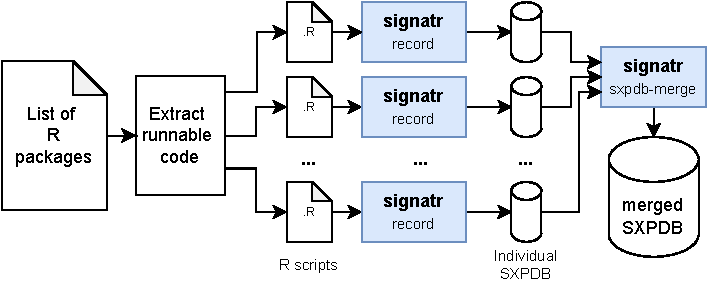
\includegraphics[width=\columnwidth]{code-and-figures/sxdb-pipeline.pdf}
    \caption{
    Database creation pipeline.
    Runnable code snippets are extracted from an input list of R packages.
    These snippets are fed in parallel to the {\tt sxpdb-create} part of \tool, which picks out values and metadata related to them (e.g., the origin of the value). 
    This creates a number of disparate databases that are merged into one database, which is referred to as the {\tt sxpdb}.
    }\label{fig:sxpdb-pipeline}
\end{figure}

\begin{figure}
    \centering
    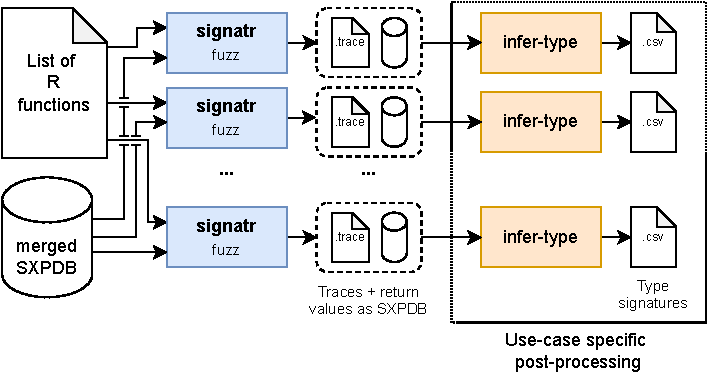
\includegraphics[width=\columnwidth]{code-and-figures/fuzz-pipeline.pdf}
    \caption{
    Fuzzing pipeline.
    The {\tt sxpdb}, along with a list of R functions to fuzz, is input to the fuzzing phase of \tool.
    The fuzzing phase fuzzes each of the functions w.r.t. the {\tt sxpdb}, which results in a collection of execution traces; these execution traces are fed to the typing phase of \tool, which infers types for arguments and outputs a list of unique call signatures.
    }\label{fig:fuzz-pipeline}
\end{figure}

\subsection{Tracer}

\AT{Quickly talk about the tracer.}

\subsection{Database of Values}

The huge amount of R values we have observed during tracing are stored in a custom-written database. 
The values are serialized, along with their \textit{origin} (defined as which package and function are they from, and whether they are an argument or return value) and some information about the value. % such as its {\tt typeof}-type and the number of times it was seen. 
Importantly, the database provides a convenient query API based on this information, which represents search parameters for the database and is comprised of the {\tt typeof}-type, \AT{list all}, and length of the value. 
% Importantly, the database provides a convenient query API: i.e., one may sample values randomly from the database according to some parameters, such as the type \PB{Should we be more precise?}, or by providing an example value on which some characteristics (again, such as the type) can be relaxed.
The database can be queried for a random value with the desired metadata (e.g., a vector of integers of length 10), or can be queried by providing an existing value along with the search parameters to be relaxed (e.g., query the database for a value similar to {\tt 42}, but relax on the length).

The value database\footnote{\url{https://github.com/PRL-PRG/sxpdb/} \PB{not anonymous.} \AT{maybe we can make a code artifact?}} is implemented in C++ with R API (in 4.5K lines of C++ code and 1.5K lines of R code).
It uses the standard R serialization to serialize R values. 
The serialized values are hashed with a quick 128-bit hash \footnote{\url{https://cyan4973.github.io/xxHash/}}. 
During tracing, one small database is generated per file, and all the small databases are then merged together; this makes it possible to parallelize the tracing phase.

\subsection{Fuzzing Technique \AT{WIP DRAFT}}

The database of values is at the core of the fuzzing approach, which is similar in spirit to mutation-based fuzzing (where instead of mutating arguments to previous calls, new argument values are selected based on previous ones).

The core of fuzzing is to generate new calls to a function $f$, and the process of choosing arguments to construct these calls is depicted in Algorithm~\ref{alg:arg-sel}.
In addition to the function $f$ and value database $db$, the algorithm considers how many query parameters to relax on ($numRelax$), as well as all of the previously seen successful calls to $f$ ($succs$).
For each parameter $p$ of $f$, the algorithm determines which parameters to relax on (this may change from one iteration to the next), finds all values that inhabited $p$ in successful calls to $f$, chooses one such value $v$, and queries the database for a value similar to $v$ in all respects, save for the parameters that are being relaxed this time.

This argument selection process is integral to the fuzzing approach itself, depicted in Algorithm~\ref{alg:fuzzer}.
First, the collection of already known successful calls to $f$ is obtained from the database $db$.
The idea in this approach is to start by selecting new arguments essentially at random by querying the database and relaxing on many parameters, and gradually reduce the number of parameters being relaxed as the fuzzer progresses.
In terms of the algorithm, the number of parameters being relaxed is reduced every $tick$, which is determined by dividing the total fuzzing budget by the number of parameters that can be relaxed ($numRelaxParameters$).
The function $f$ will be fuzzed for as long as the budget allows, and initially all database parameters will be relaxed.
Arguments for a new call to $f$ are generated through the approach depicted in Algorithm~\ref{alg:arg-sel} ($getNewArgs$), the call is performed, and the results are saved in $res$.
If there were no errors, warnings, or crashes, then the successful call is added to the list of successful calls $succs$, and iteration continues until the budget is exhausted.

\begin{algorithm}
\caption{Selecting Arguments for New Call}\label{alg:arg-sel}
\begin{algorithmic}[1]
\Procedure{getNewArgs}{$f,numRelax,db,succs$}
\State{$params \gets getParameters(f)$}
\For{$p$ in $params$}
\LineComment{relax on $numRelax$ parameters}
\State{$relax \gets pickSome(relaxParameters, numRelax)$}
\LineComment{get all values that $p$ had in successful calls to $f$}
\State{$seed \gets getArgsFor(p, succs)$}
\LineComment{choose one at random}
\State{$v \gets pickOne(seed)$}
\LineComment{sample a similar value from the database}
\State{$args[p] \gets sampleSimilar(v, db, relax)$}
\EndFor
\State \textbf{return} $args$\Comment{the args for the new call}
\EndProcedure
\end{algorithmic}
\end{algorithm}

\begin{algorithm}
\caption{Fuzzing}\label{alg:fuzzer}
\begin{algorithmic}[1]
\Procedure{fuzzWithDB}{$f,db,budget$}
\State $succs \gets getSuccessfulCalls(f, db)$
\State $tick \gets budget / numRelaxParameters$
\State $relaxThisTime \gets numRelaxParameters$
\State $i\gets 1$
\While{$i\not=budget$}
\LineComment{gradually relax on fewer parameters}
\If{$i \bmod tick = 0$}
\State $relaxThisTime \gets relaxThisTime - 1$
\EndIf
\State{$args \gets getNewArgs(f,relaxThisTime, db, succs)$}
\State{$res \gets call(f, args)$}
\LineComment{add successful call to $succs$}
\If{no warnings, errors, crashes in $res$}
\State{$succs \gets succs + res$}
\EndIf
\State $i\gets i+1$
\EndWhile\label{endfuzzloop}
\State \textbf{return} $succs$\Comment{the successful calls to $f$}
\EndProcedure
\end{algorithmic}
\end{algorithm}

\subsection{Typing Successful Traces}

Once the fuzzer has finished obtaining successful function call traces, the types corresponding to the successful calls are determined.
This is the stage where a user can define their type system, which is input as two functions: one to infer the type of some value $v$, and another to take two types $t_1$ and $t_2$ and judge whether or not they can be simplified (e.g., determine if $t_1$ is a subtype of $t_2$, $t_1 <: t_2$).
This helps determine the set of \textit{unique} call signatures for a function, as two calls with different values that have the same type can be collapsed at this stage.
For example, say the identity function {\tt id} was called with {\tt 2} and {\tt 4}; the types of each of those calls is $int \rightarrow int$, and so they would be collapsed together. 
% The current implementation of \tool uses {\tt contractr}~\cite{turcotte2020designing} to infer types, and uses the subtyping rules described in that paper.

The fuzzing approach is implemented in a tool called \tool, written in R and C++, and is available as an R package.

\subsection{Threats to Validity}


\FK{If we decide to keep this then here we should probably discuss the possible problems with fuzzing.}

\section{Assessment}
\label{sec:assessment}

The main motivation for building \tool was to have a tool that can generate successful calls to R functions, \emph{in addition} to what we can record by running the available executable code from R packages.
Therefore, to assess the usefulness of \tool we need to answer \emph{how many additional successful calls can \tool generates?}.

We ran all of our experiments on Intel Xeon 6140, 2.30GHz with 72 cores and 256GB of RAM running Ubuntu 18.04.

\subsection{Fuzzing user functions}

We base the experiment on the same corpus as we used in the \typer paper (412 packages, 17.4K public functions).
First, we created a \sxpdb for the fuzzer.
For this we used the extracted runnable code from the corpus packages which consists of \DBNumSourceFiles files containing \DBSourceLinesOfCodeRnd lines of R code (excluding comments and new lines).
Generating the database took \TODO{XXX - @pierre} and takes \DBFileSize of disk space.
It contains \DBValuesRnd unique values recorded from \DBNumCallsRnd calls to \DBNumFunctionsRnd functions in \DBNumPackages packages.
\FK{Info about value distribution? A pie chart?}

With this database, we fuzzed \UFNumFunctions functions from \UFNumPackages packages, a subset of the original corpus.
Each function was run \UFTracingBudget times, taking it 36 hours while fuzzing 32 functions in parallel\footnote{Trying bigger number resulted in tasks being killed due to running out of memory.}.

In total we made \UFNumTracesRnd calls (\UFTracesSize of traces and \UFTracesReturnDbsSize). Out of that, \UFRatioSuccessTraces were successful, resulting in \UFNumSuccessTraces traces of \UFNumSuccessFunctions functions coming from \UFNumSuccessPackages packages.
The vast majority of errors were exceptions, but in \UFNumOfCrashedRSessions cases, R processed crashed.

\FK{Report the stringi bug that was fixed}




% how often R crashed

\begin{figure}
    \centering
    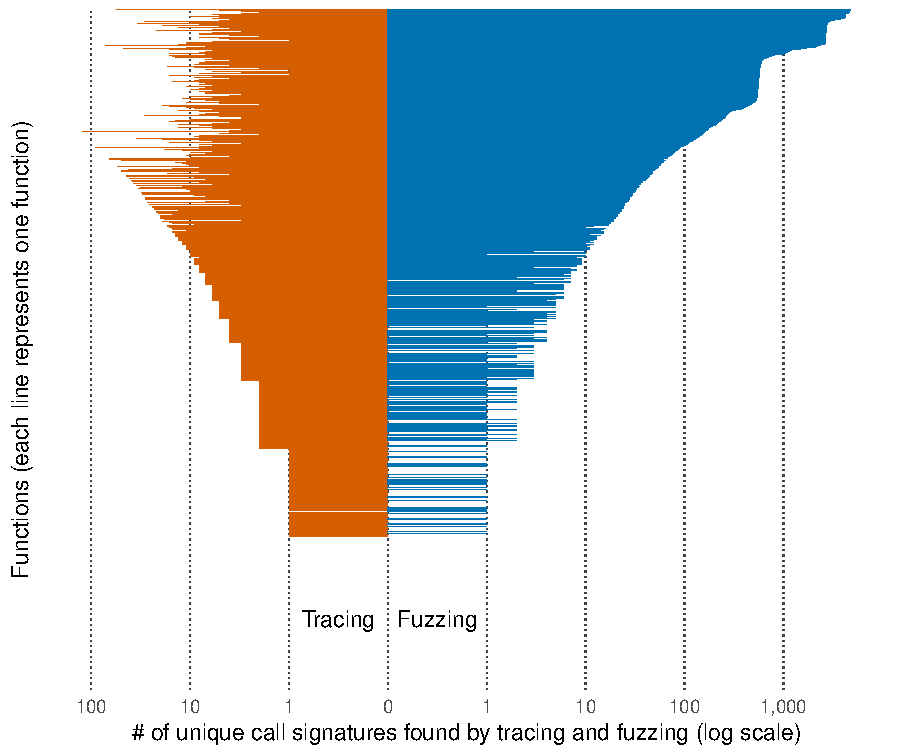
\includegraphics[width=\columnwidth]{code-and-figures/uf-call-signatures.pdf}
    \caption{
        Number of call signatures obtained by fuzzing in addition to tracing. Each line represents one function.
        \FK{an alternative would be to show proportionally how many out of all sigantures come from fuzzing / traing - no need for log scale then}
    }\label{fig:sxpdb-pipeline}
\end{figure}

\subsection{Fuzzing stdlib}

%
It took 6 hours with all functions fuzzed in parallel.


% a table with function and number of type signatres

\section{Conclusions}
\label{sec:conclusions}

%%
%% The next two lines define the bibliography style to be used, and
%% the bibliography file.
\bibliographystyle{ACM-Reference-Format}
\bibliography{fuzzing}

\appendix

\section{\tool demonstration}

The following is a short demo of the basic \tool functionality, \Ie how to create the value database by running R code and then use it to fuzz function type traces.
We will be using the command line interface but the same is available directly in R and thus directly usable from pipeline frameworks such as targets.

\FK{Once I have it up and running I will split the listings into multiple, fix the new lines and add the description to each of the command.}

\begin{lstlisting}
$ cat example-1.R
...

$ cat example-2.R
...

$ ls example*.R | parallel signatr record --from '{1}' --db '{1.-sxpdb}'
...

$ ls -l
...

$ signatr sxpdb-info example-1-sxpdb
...

$ signatr sxpdb-info example-2-sxpdb
...

$ signatr sxpdb-merge --output merged-sxpdb example-*-sxpdb
...

$ signatr sxpdb-info merged-sxpdb
...

$ signatr fuzz --target "base:::`+`" --db merged-sxpdb --budget 100 --output traces
...

$ ls -lh fuzz
...

$ signatr type --traces traces --output types.csv
...

$ wc -l types.csv
...

$ head -10 types.csv
...

$ R -e 'read.csv("type.csv")["signature"] |> unique |> length'
...

\end{lstlisting}

\end{document}
\endinput
